
%% Style 45


\cxset{
 name=,
 numbering=none,
 number font-size=,
 number before=,
 number after=,
 number position=rightname,
 chapter color=black,
 chapter font-size=,
 chapter before=\thinrule,
 chapter after=\vskip20pt ,
 number color=\color{black!80},
 title font-family=\rmfamily,
 title font-color=\color{black!80},
 title font-weight=,
 title font-size=\huge,
 title font-shape=\upshape,
 title beforeskip=,
 title after=\par\vspace*{20pt},
 title afterskip=\vspace*{20pt},
 header style=empty,
 author block format=\normalfont\upshape\LARGE,
 author block=true,
 section align=\raggedright,
 section indent=0pt,
 section font-weight=\bfseries,
 section font-size=\LARGE}

\addauthors{D.T.Potts}
\chapter{A Short Introduction\\ to Style Forty Five\\ including the addition\\of an author}

\section{Introduction}
This is an unusual book with a rather unique style. The vertical rule is simple and breaks the monotony of a book that is heavy on text.
\begin{figure}[ht]
\centering
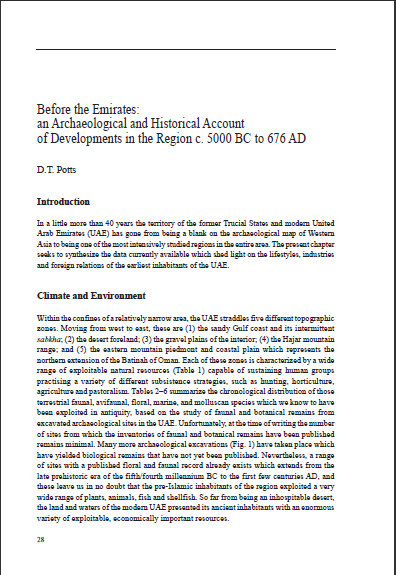
\includegraphics[width=0.6\textwidth]{./chapters/chapter45}
\end{figure}


UNITED ARAB EMIRATES
a new perspective
Edited by
IBRAHIM AL ABED
PETER HELLYERTrident Press Ltd
Layout and design,1997, 2001 Trident Press Ltd,UK.




%% Style 46

\cxset{,
 name=CHAPTER,
 numbering=arabic,
 number font-size=\Large,
 number before={},
 number position=rightname,
 chapter color={black!80},
 chapter font-size=\Large,
 chapter before=\par\hfill\hfill,
 number after=,
 chapter after=\vskip20pt ,
 number color=\color{black!80},
 title font-family=\itshape,
 title font-color=\color{black!80},
 title font-weight=,
 title font-size=\LARGE,
 title beforeskip=\hfill,header style=empty}

\section{Introduction to Style 46}


This is an unusual book with a rather unique style. The vertical rule is simple and breaks the monotony of a book that is heavy on text.
\begin{figure}[ht]
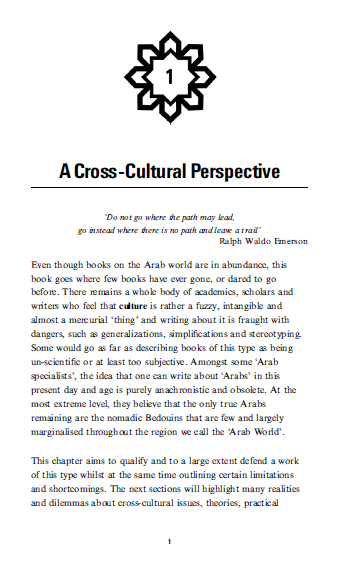
\includegraphics[width=0.45\textwidth]{./chapters/chapter46}
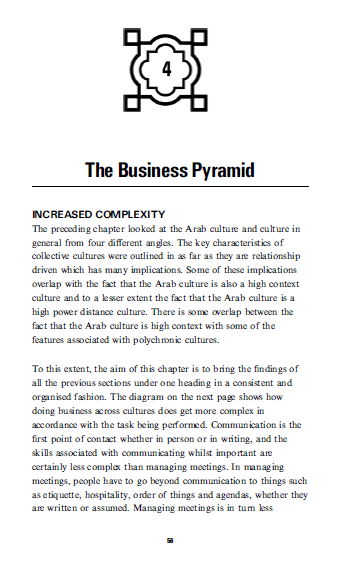
\includegraphics[width=0.45\textwidth]{./chapters/chapter46a}
\end{figure}

Understanding the Arab Culture a cross-cultural guide, second edition, published by How To Content, Dr Jehad Al-Omari,2008.

%% Style 46
\def\anornament{%
\begin{tikzpicture}[decoration={markings,
  mark=between positions 0 and 1 step 8pt
  with { \draw [fill=black] (0,0) circle [radius=1pt];}}]
\path[postaction={decorate}] (0,0) to (15,0);
\end{tikzpicture}}


\cxset{style46/.style={%
 name=CHAPTER,
 numbering=arabic,
 number font-size=\Large,
 number before={},
 number position=rightname,
 chapter color={black!80},
 chapter font-size=\Large,
 chapter before=\par\hfill,
 number after=,
 chapter after=\hfill\hfill\par,
 number color=\color{black!80},
 title font-family=\rmfamily,
 title font-shape=\upshape,
 title font-color=\color{black!80},
 title font-weight=,
 title font-size=\LARGE,
 title before=\par\anornament\par \centering,
 title after= \vskip-10pt\anornament\par\vspace*{10pt},
 title beforeskip=,
 title afterskip=\vspace*{30pt},
 author block format=\large,
 header style=empty}}

\cxset{style46}
\addauthors{Jonathan Taylor}
\chapter{INTRODUCTION TO STYLE\\ FORTY SIX }\label{STYLE:46}

This is an unusual book with a rather unique style. The book is heavy on text and I introduced it to show the possibilities of ornaments with TikZ. The rule is made out of tikz decorations as per an answer on tex.sx.
\begin{figure}[ht]
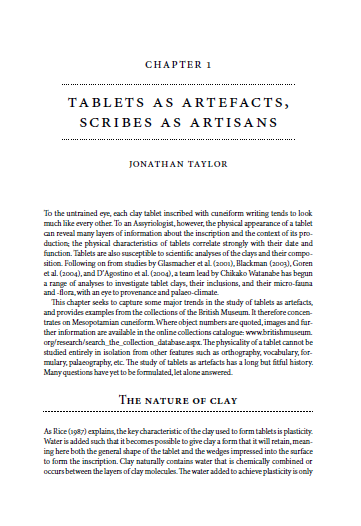
\includegraphics[width=0.48\textwidth]{./chapters/chapter48}\hfill
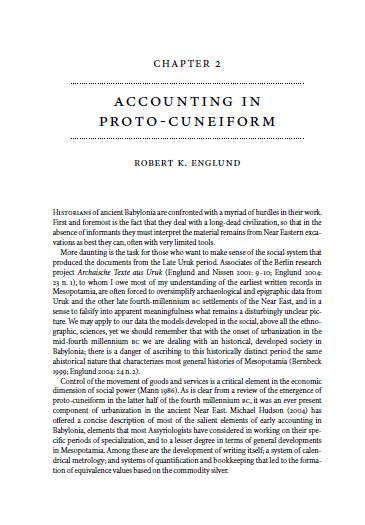
\includegraphics[width=0.48\textwidth]{./chapters/chapter48a}
%\caption{Style 48 from the Oxford Handbook of Cuneiform Culture.}
\end{figure}


